\chapter{Tables and graphs}
\label{ch:tables_and_graphs}

\section{Use cases}
\label{sec:use_cases_appendix}

Below are the different use cases created during the requirements elicitation process.

\subsection{Use case 2 - Topic handling}
\label{subsec:requirements_engineering-use_cases-topic_handling}

This use case describes how an administrator can delete topics. The administrator must be able to delete one or all topics.

\begin{table}[ht!]
\begin{minipage}{.5\textwidth}
\centering
\resizebox{\textwidth}{!}{
\begin{tabular}{|l|p{5cm}|}
\hline
\textbf{Use case ID} & U2 \\ \hline
\textbf{Use case Name} & Topic handling \\ \hline
\textbf{Description} & Admin should be able to delete topics.  \\ \hline
\textbf{Pre conditions} & The admin is logged in and there exists one or more topics. \\ \hline
\textbf{Standard flow} & \begin{enumerate}
\item Click the topics pane.
\item Click delete button on the topic.
\item Alternatives: \begin{enumerate}
    \item Delete one topic.
    \item Delete all topics.
\end{enumerate}
\end{enumerate} \\ \hline
\textbf{Alternative flow} &  \\ \hline
\textbf{Post conditions} & Topics are deleted from the broker.  \\ \hline
\end{tabular}
}
\caption{Use case 2 - Topic handling}
\label{uc2}
\end{minipage}
\hfill
\begin{minipage}{.4\textwidth}
\centering
\begin{center}
    \makebox[\textwidth]{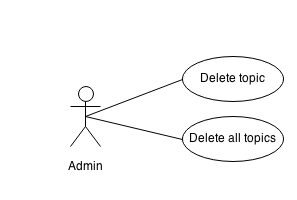
\includegraphics[width=\textwidth]{fig/usecase/usecase_u2_topic_mapping.png}}
    \caption{U2 - Topic handling}
    \label{fig:u2}
\end{center}
\end{minipage}
\end{table}

\clearpage

\subsection{Use case 3 - Server information}
\label{subsec:requirements_engineering-use_cases-server_information}

This use case describes how an administrator can view information about the server. This includes server statistics and message brokering statistics. 

\begin{table}[ht!]
\centering
\begin{tabular}{|l|p{5cm}|}
\hline
\textbf{Use case ID} & U3 \\ \hline
\textbf{Use case Name} & Server information. \\ \hline
\textbf{Description} & As an admin I would like to see information and status about the server.  \\ \hline
\textbf{Pre conditions} & The admin is logged in.\\ \hline
\textbf{Standard flow} & \begin{enumerate}
\item Click the pane of interest.
\item Read information on the pane of interest.  
\end{enumerate} \\ \hline
\textbf{Alternative flow} & \\ \hline
\textbf{Post conditions} & The admin has seen the information. \\ \hline
\end{tabular}
\caption{Use case 3 - Server information}
\label{uc3}
\end{table}

\begin{center}
  \begin{figure}[ht!]
    \makebox[\textwidth]{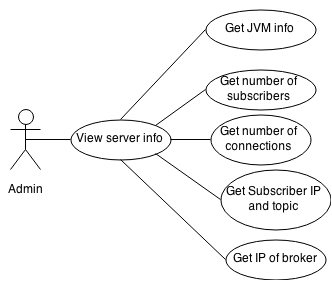
\includegraphics[width=6cm]{fig/usecase/usecase_v3_serverinfo.png}}
    \caption{U3 - Server information}
    \label{fig:u3}
  \end{figure}
\end{center}

\clearpage

\subsection{Use case 4 - Log in}
\label{subsec:requirements_engineering-use_cases-log_in}

The following describes the log in procedure. The group concluded that no other functions were needed than a simple username and password log in function. Recover password were not included due to there being little to no persistent data in the database. Thus, a new instance could be initiated instead.

\begin{table}[ht!]
\centering
\begin{tabular}{|l|p{5cm}|}
\hline
\textbf{Use case ID} & U2 \\ \hline
\textbf{Use case Name} & Log in \\ \hline
\textbf{Description} & As an Admin I would like to log in to the admin console. \\ \hline
\textbf{Pre conditions} & The admin is not logged in. \\ \hline
\textbf{Standard flow} & \begin{enumerate}
\item Inserts username and password.
\item Clicks "Log in".
\item Enter the admin console. 
\end{enumerate} \\ \hline
\textbf{Alternative flow} & \begin{description}
\item[2A:] The username or password is wrong. \begin{enumerate}
\item Redirect user to front page.
\item Display error message.
\end{enumerate}
\end{description} \\ \hline
\textbf{Post conditions} & Admin logged in. \\ \hline
\end{tabular}
\caption{Use case 4 - Log in}
\label{uc4}
\end{table}

\begin{center}
  \begin{figure}[ht!]
    \makebox[\textwidth]{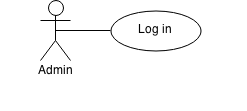
\includegraphics[width=6cm]{fig/usecase/usecase1.png}}
    \caption{U4 - Log in}
    \label{fig:u4}
  \end{figure}
\end{center}

\subsection{Use case 5 - Message sending}
\label{subsec:requirements_engineering-use_cases-message_sending}

This use case attempts to capture the process of sending messages over the system. This only captures a simplified version of the message sending. Some variations occur from protocol to protocol.

\begin{table}[ht!]
\centering
\begin{tabular}{|l|p{5cm}|}
\hline
\textbf{Use case ID} & U5 \\ \hline
\textbf{Use case Name} & Message sending \\ \hline
\textbf{Description} & User should be able to send a message over a protocol.  \\ \hline
\textbf{Pre conditions} &  \\ \hline
\textbf{Standard flow} & \begin{enumerate}
\item Register as a publisher on a topic.
\item Send the message.
\end{enumerate} \\ \hline
\textbf{Alternative flow} & \begin{enumerate}
\item [1A:] Topic is protected.
\item User registers as publisher with username and password.
\end{enumerate} \\ \hline
\textbf{Post conditions} & Message is sent.  \\ \hline
\end{tabular}
\caption{Use case 5 - Message sending}
\label{uc5}
\end{table}

\begin{center}
  \begin{figure}[ht!]
    \makebox[\textwidth]{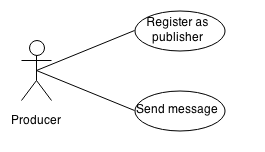
\includegraphics[width=6cm]{fig/usecase/fig44.png}}
    \caption{U5 - Message sending}
    \label{fig:u5}
  \end{figure}
\end{center}

\clearpage

\subsection{Use case 6 - Message Receiving}
\label{subsec:requirements_engineering-use_cases-message_recieving}

This use case attempts to capture the process of receiving messages over the system. This only captures a simplified version of the message retrieval. Some variations occur from protocol to protocol.

\begin{table}[ht!]
\centering
\begin{tabular}{|l|p{5cm}|}
\hline
\textbf{Use case ID} & U6 \\ \hline
\textbf{Use case Name} & Receiving messages. \\ \hline
\textbf{Description} & User should be able to receive a message over a protocol.  \\ \hline
\textbf{Pre conditions} & The message is sent. \\ \hline
\textbf{Standard flow} & \begin{enumerate}
\item Register as a subscriber on a topic.
\item Receive the message.
\end{enumerate} \\ \hline
\textbf{Alternative flow} & \\ \hline
\textbf{Post conditions} & Message has been received.  \\ \hline
\end{tabular}
\caption{Use case 6 - Message retrieval}
\label{uc6}
\end{table}

\begin{center}
  \begin{figure}[ht!]
    \makebox[\textwidth]{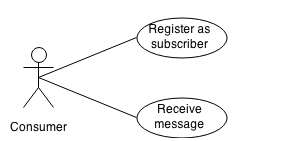
\includegraphics[width=6cm]{fig/usecase/fig45.png}}
    \caption{U6 - Message retrieval}
    \label{fig:u6}
  \end{figure}
\end{center}
\clearpage

\subsection{Use case 7 - Subscribe with WSN}
\label{subsec:requirements_engineering-use_cases-sub_wsn}

This use case attempts to capture the process of subscribing to a topic using the WSN protocol. 

\begin{table}[ht!]
\centering
\begin{tabular}{|l|p{5cm}|}
\hline
\textbf{Use case ID} & U7 \\ \hline
\textbf{Use case Name} & Subscribe with WSN. \\ \hline
\textbf{Description} & A consumer should be able to subscribe to a topic using the WSN protocol.  \\ \hline
\textbf{Pre conditions} & OKSE broker is up and running. \\ \hline
\textbf{Standard flow} & \begin{enumerate}
\item Send subscription request to OKSE.
\end{enumerate} \\ \hline
\textbf{Alternative flow} & \\ \hline
\textbf{Post conditions} & The consumer is now subscribed to the requested topic.  \\ \hline
\end{tabular}
\caption{Use case 7 - Subscribe with WSN}
\label{uc7}
\end{table}

\begin{center}
  \begin{figure}[ht!]
    \makebox[\textwidth]{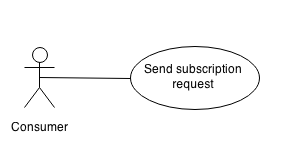
\includegraphics[width=6cm]{fig/usecase/usecase_u7_sub_wsn}}
    \caption{U7 - Subscribe with WSN}
    \label{fig:u7}
  \end{figure}
\end{center}
\clearpage

\subsection{Use case 8 - Register as a publisher on a topic with WSN}
\label{subsec:requirements_engineering-use_cases-reg_pub_wsn}

Use case showing how to register as a publisher on a topic using the WSN protocol 

\begin{table}[ht!]
\centering
\begin{tabular}{|l|p{5cm}|}
\hline
\textbf{Use case ID} & U8 \\ \hline
\textbf{Use case Name} & Register producer WSN. \\ \hline
\textbf{Description} & A client should be able to register as publisher on a topic with the WSN protocol.  \\ \hline
\textbf{Pre conditions} & OKSE broker is up and running. \\ \hline
\textbf{Standard flow} & \begin{enumerate}
\item Send request to OKSE.
\item Receive registration confirmation.
\end{enumerate} \\ \hline
\textbf{Alternative flow} & \\ \hline
\textbf{Post conditions} & Client is now registered as a publisher on the requested topic. 
  \\ \hline
\end{tabular}
\caption{Use case 8 - Register producer WSN}
\label{uc8}
\end{table}

\begin{center}
  \begin{figure}[ht!]
    \makebox[\textwidth]{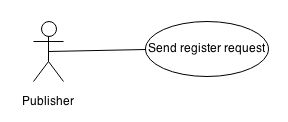
\includegraphics[width=6cm]{fig/usecase/usecase_u8_pubreg_wsn}}
    \caption{U8 - Register producer WSN}
    \label{fig:u8}
  \end{figure}
\end{center}

\clearpage

\subsection{Use case 9 - Unsubscribe with WSN}
\label{subsec:requirements_engineering-use_cases-unsub_wsn}

Use case showing how to unsubscribe from a topic using the WSN protocol. 

\begin{table}[ht!]
\centering
\begin{tabular}{|l|p{5cm}|}
\hline
\textbf{Use case ID} & U9 \\ \hline
\textbf{Use case Name} & Unsubscribe with WSN. \\ \hline
\textbf{Description} & A user must be able to unsubscribe for a topic using the WSN protocol.  \\ \hline
\textbf{Pre conditions} & OKSE broker is up and running. The user has an active subscription on the topic which the user wants to 	unsubscribe from. \\ \hline
\textbf{Standard flow} & \begin{enumerate}
\item Send unsubscribe request to OKSE.
\item Receive unsubscribe confirmation.
\end{enumerate} \\ \hline
\textbf{Alternative flow} & \\ \hline
\textbf{Post conditions} & The user is now unsubscribed from requested topic and will no longer receive messages sent on that topic. 
  \\ \hline
\end{tabular}
\caption{Use case 9 - Unsubscribe from topic WSN}
\label{uc9}
\end{table}

\begin{center}
  \begin{figure}[ht!]
    \makebox[\textwidth]{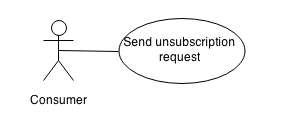
\includegraphics[width=6cm]{fig/usecase/usecase_u9_unsub_wsn}}
    \caption{U9 - Unsubscribe from topic WSN}
    \label{fig:u9}
  \end{figure}
\end{center}

\clearpage

\subsection{Use case 10 - Unregister as a publisher on a topic wih WSN.}
\label{subsec:requirements_engineering-use_cases-unreg_pub}

Use case showing how to unregister as a publisher using the WSN protocol. 

\begin{table}[ht!]
\centering
\begin{tabular}{|l|p{5cm}|}
\hline
\textbf{Use case ID} & U10 \\ \hline
\textbf{Use case Name} & Unregister as publisher with WSN. \\ \hline
\textbf{Description} & A user must be able to unregister as a publisher on a topic using the WSN protocol.  \\ \hline
\textbf{Pre conditions} & OKSE broker is up and running. The user is registered as a publisher on the topic which the user wants to unsubscribe from.  \\ \hline
\textbf{Standard flow} & \begin{enumerate}
\item Send unregister request to OKSE.
\item Receive unregister confirmation.
\end{enumerate} \\ \hline
\textbf{Alternative flow} & \\ \hline
\textbf{Post conditions} & The user is now unregistered as a publisher on the requested topic. 
  \\ \hline
\end{tabular}
\caption{Use case 10 - Unregister as publisher using WSN}
\label{uc10}
\end{table}

\begin{center}
  \begin{figure}[ht!]
    \makebox[\textwidth]{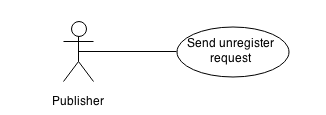
\includegraphics[width=6cm]{fig/usecase/usecase_u10_pubunreg_wsn}}
    \caption{U10 - Unregister as publisher using WSN}
    \label{fig:u10}
  \end{figure}
\end{center}

\clearpage

\subsection{Use case 11 - Retrieve the latest message on a topic using the GetCurrentMessage function with WSN.}
\label{subsec:requirements_engineering-use_cases-get_message_wsn}

Use case showing how to retrieve the latest message on a topic using the GetCurrentMessage function.


\begin{table}[ht!]
\centering
\begin{tabular}{|l|p{5cm}|}
\hline
\textbf{Use case ID} & U11 \\ \hline
\textbf{Use case Name} & Get latest message on topic using WSN.\\ \hline
\textbf{Description} & A user must be able to get the last message sent on a topic using the WSN protocol\\ \hline
\textbf{Pre conditions} & OKSE broker is up and running. There is a message to retrieve.\\ \hline
\textbf{Standard flow} & \begin{enumerate}
\item Send request using GetCurrentMessage to OKSE using WSN.
\item Receive last message sent on requested topic.
\end{enumerate} \\ \hline
\textbf{Alternative flow} & \\ \hline
\textbf{Post conditions} & User now has local copy of last message sent on requested topic  
  \\ \hline
\end{tabular}
\caption{Use case 11 - GetCurrentMessage function with WSN}
\label{uc11}
\end{table}

\begin{center}
  \begin{figure}[ht!]
    \makebox[\textwidth]{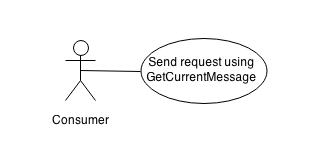
\includegraphics[width=6cm]{fig/usecase/usecase_u11_lastmess_wsn}}
    \caption{U11 - GetCurrentMessage function with WSN}
    \label{fig:u11}
  \end{figure}
\end{center}

\clearpage

\subsection{Use case 12 - Renew subscription using the WSN protocol}
\label{subsec:requirements_engineering-use_cases-renew_sub_wsn}

Use case showing the steps involved in renewing subscription on topic with WSN. 

\begin{table}[ht!]
\centering
\begin{tabular}{|l|p{5cm}|}
\hline
\textbf{Use case ID} & U12 \\ \hline
\textbf{Use case Name} & Renew subscription using WSN protocol.\\ \hline
\textbf{Description} & A user should be able to renew subscription on a requested topic using WSN protocol.\\ \hline
\textbf{Pre conditions} & OKSE is up and running. The user has an active subscription on the topic which he/she wants to renew.\\ \hline
\textbf{Standard flow} & \begin{enumerate}
\item Send request to OKSE with new timeout date. 
\item Receive confirmation from OKSE with updated subscription timeout date.
\end{enumerate} \\ \hline
\textbf{Alternative flow} & \\ \hline
\textbf{Post conditions} & The user will have a updated timeout date for the subscription on the requested topic.\\ \hline
\end{tabular}
\caption{Use case 12 - Renew subscription using WSN}
\label{uc12}
\end{table}

\begin{center}
  \begin{figure}[ht!]
    \makebox[\textwidth]{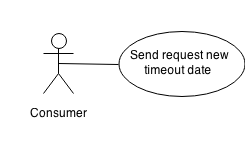
\includegraphics[width=6cm]{fig/usecase/usecase_u12_renewsub_wsn}}
    \caption{U12 - Renew subscription using WSN}
    \label{fig:u12}
  \end{figure}
\end{center}

\clearpage

\subsection{Use case 13 - Pause subscription using the WSN protocol}
\label{subsec:requirements_engineering-use_cases-pause_sub_wsn}

Use case showing the steps involved in pausing subscription on topic with WSN. 

\begin{table}[ht!]
\centering
\begin{tabular}{|l|p{5cm}|}
\hline
\textbf{Use case ID} & U13 \\ \hline
\textbf{Use case Name} & Pause subscription using WSN protocol.\\ \hline
\textbf{Description} & The user should be able to pause a subscription on a requested topic using the WSN protocol. \\ \hline
\textbf{Pre conditions} & OKSE is up and running. User must have active subscription on the topic which he/she wants to pause\\ \hline
\textbf{Standard flow} & \begin{enumerate}
\item Send request to OKSE. 
\item Receive confirmation from OKSE.
\end{enumerate} \\ \hline
\textbf{Alternative flow} & \\ \hline
\textbf{Post conditions} & Subscription is now on pause. User will no longer receive messages sent on that topic. Subscription is not removed from OKSE\\ \hline
\end{tabular}
\caption{Use case 13 - Pause subscription using WSN}
\label{uc13}
\end{table}

\begin{center}
  \begin{figure}[ht!]
    \makebox[\textwidth]{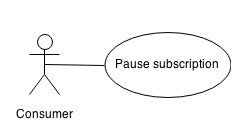
\includegraphics[width=6cm]{fig/usecase/usecase_u13_pause_wsn}}
    \caption{U13 - Pause subscription using WSN}
    \label{fig:u13}
  \end{figure}
\end{center}

\clearpage

\subsection{Use case 14 - Resume subscription using the WSN}
\label{subsec:requirements_engineering-use_cases-resume_sub_wsn}

Use case showing the steps involved in resuming a paused subscription on topic with WSN. 

\begin{table}[ht!]
\centering
\begin{tabular}{|l|p{5cm}|}
\hline
\textbf{Use case ID} & U14 \\ \hline
\textbf{Use case Name} & Resume subscription with WSN protocol\\ \hline
\textbf{Description} & The user should be able to resume a subscription on a topic which previously was paused. \\ \hline
\textbf{Pre conditions} & OKSE is up and running. User has a paused subscription on the topic which he/she wants to resume. \\ \hline
\textbf{Standard flow} & \begin{enumerate}
\item Send request to OKSE
\item Receive confirmation from OKSE	
\end{enumerate} \\ \hline
\textbf{Alternative flow} & \\ \hline
\textbf{Post conditions} & The subscription on the requested topic is resumed. The user will now receive messages sent on the topic which the user resumed subscription on.  \\ \hline
\end{tabular}
\caption{Use case 14 - Resume subscription with WSN}
\label{uc14}
\end{table}

\begin{center}
  \begin{figure}[ht!]
    \makebox[\textwidth]{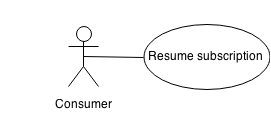
\includegraphics[width=6cm]{fig/usecase/usecase_u14_resume_wsn}}
    \caption{U14 - Resume subscription with WSN}
    \label{fig:u14}
  \end{figure}
\end{center}

\clearpage

\subsection{Use case 15 - Multiple notifications, single Notify using WSN }
\label{subsec:requirements_engineering-use_cases-}

Use case showing the steps involved in sending a Notify to subscribers containing more than one notification using WSN. 

\begin{table}[ht!]
\centering
\begin{tabular}{|l|p{5cm}|}
\hline
\textbf{Use case ID} & U15 \\ \hline
\textbf{Use case Name} & Multiple notification single Notify\\ \hline
\textbf{Description} & The user must be able to send multiple notification messages in a single Notify using WSN\\ \hline
\textbf{Pre conditions} & OKSE is up and running. Subscribers on the topic which the Notify is sent to. \\ \hline
\textbf{Standard flow} & \begin{enumerate}
\item Send one Notify containing multipe notifications
\end{enumerate} \\ \hline
\textbf{Alternative flow} & \\ \hline
\textbf{Post conditions} & Subscribers receive more than one Notify on the topic which the notification was sent on\\ \hline
\end{tabular}
\caption{Use case 15 - Multiple notifications}
\label{uc15}
\end{table}

\begin{center}
  \begin{figure}[ht!]
    \makebox[\textwidth]{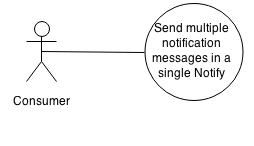
\includegraphics[width=6cm]{fig/usecase/usecase_u15_notify_wsn.png}}
    \caption{U15 - Multiple notifications}
    \label{fig:u15}
  \end{figure}
\end{center}

\clearpage

\subsection{Use case 16 - Subscribe with AMQP protocol}
\label{subsec:requirements_engineering-use_cases-}

Use case showing the steps involvedin subscribing to a topic using the AMQP protocol.   

\begin{table}[ht!]
\centering
\begin{tabular}{|l|p{5cm}|}
\hline
\textbf{Use case ID} & U16 \\ \hline
\textbf{Use case Name} & AMQP subscribe\\ \hline
\textbf{Description} & The user must be able to subscribe to a topic using the AMQP protocol. \\ \hline
\textbf{Pre conditions} & OKSE must be up and running. \\ \hline
\textbf{Standard flow} & \begin{enumerate}
\item Connect to the server.
\end{enumerate} \\ \hline
\textbf{Alternative flow} & \\ \hline
\textbf{Post conditions} & The user is now connected and subscribed to the topic of choice. Can now receive messages on that topic. \\ \hline
\end{tabular}
\caption{Use case 16 - AMQP subscribe}
\label{uc16}
\end{table}

\begin{center}
  \begin{figure}[ht!]
    \makebox[\textwidth]{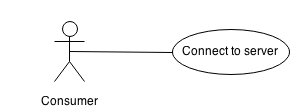
\includegraphics[width=6cm]{fig/usecase/usecase_u16_sub_amqp.png}}
    \caption{U16 - AMQP subscribe}
    \label{fig:u16}
  \end{figure}
\end{center}

\clearpage

\section{Testing}
\label{sec:appendix-testing}

\subsection{Integration testing test cases}

\begin{table}[ht!]
\tiny
\begin{tabular}{|m{0.5cm}|m{1.5cm}|m{1.5cm}|m{3cm}|m{3cm}|m{1.5cm}|}
\hline
\rowcolor{lightgray}
\textbf{ID} & \textbf{Service/Protocol} & \textbf{Method} & \textbf{Procedure} & \textbf{Expected} & \textbf{Result}\\ \hline
IT1.1 & CoreService & boot & Start the Application & Thread running and all registered services alive & Success \\ \hline
IT1.2 & CoreService & stop & Stop the Application & All registered services shut down and threads killed. Invoked flags set to false. CoreService thread removed and invoked flag set to false. & Success \\ \hline
IT1.3 &CoreService & execute & Create and insert a runnable job to the executor service using the execute method & Job successfully performed & Success \\ \hline
IT1.4 & CoreService & registerService & Initialize a stub abstractcoreservice and register it to the CoreService & Stub service is correctly registered & Success \\ \hline
IT1.5 & CoreService & removeService & Perform IT1.4 and then remove the service again & Service correctly removed & Success \\ \hline
IT1.6 & CoreService & addProtocolServer & Register the DummyProtocolServer & DummyProtocolServer correctly added to list of protocol servers & Success \\ \hline
IT1.7 & CoreService & removeProtocolServer & Perform IT1.6 and then remove the protocol server again & Protocol server correctly removed & Success \\ \hline
IT1.8 & CoreService & getTotalRequests FromProtocolServers & Perform a request using DummuProtocolServer and verify counter increment in admin panel & Request counter incremented by 1 per request & Success \\ \hline
IT1.9 & CoreService & getTotalMessages RecievedFromProtocolServers & Increment the DummyProtocol's recieved messages field & Messages recieved counter incremented by 1 per message & Success \\ \hline
IT1.10 & CoreService & getTotalMessages SentFromProtocolServers & Increment the DummyProtocol's sent messages field & Messages sent counter incremented by 1 per message & Success \\ \hline
IT1.11 & CoreService & getTotalBadRequests FromProtocolServers & Write jibberish using the DummyProtocol telnet command interface & Bad requests counter incremented by 1 per bad request sent & Success \\ \hline
IT1.12 & CoreService & getTotalErrors FromProtocolServers & Increment the DummyProtocol's total errors field & Total errors counter incremented by 1 per error & Success \\ \hline
IT1.13 & CoreService & getAllProtocolServers & Perform IT6.1 and verify that it is returned from the method & Set of registered protocol servers increased by 1 during registry, and DummyProtocolServer included in the shallow copy hash set returned. & Success \\ \hline
IT1.14 & CoreService & getProtocolServer & Perform IT6.1 and then provide the Class type of the DummyProtocolServer as an argument. & The instance of DummyProtocolServer successfully returned & Success \\ \hline
IT1.15 & CoreService & stopAllProtocol Servers & Call the method from test class & All protocol servers gracefully shut down, their threads removed and invoked flag set to false. & Success \\ \hline
IT1.16 & CoreService & bootCoreServices & Perform 1.4 twice using 2 different stubs. Then call the method. & Both registered stub services booted successfully in their own thread, with run and invoked flags set to true. & Success \\ \hline
IT1.17 & CoreService & bootProtocolServers & Perform IT1.6 then call the method & DummyProtocoLServer successfully booted in its own thread, with run and invoked flags set to true. & Success \\ \hline
IT1.18 & CoreService & registerListenerSupport ForAllCoreServices & Perform IT1.4 with debug output in its registerListenerSupport method. Then invoke the test method & Debug output successfully displayed when method is invoked. & Success \\ \hline
\end{tabular}
\caption{Integration Testing - Test Cases - CoreService}
\label{table:integration-testing-cases}
\end{table}

\clearpage

\begin{table}[ht!]
\tiny
\begin{tabular}{|m{0.5cm}|m{1.5cm}|m{1.5cm}|m{3cm}|m{3cm}|m{1.5cm}|}
\hline
\rowcolor{lightgray}
\textbf{ID} & \textbf{Service/Protocol} & \textbf{Method} & \textbf{Procedure} & \textbf{Expected} & \textbf{Result}\\ \hline
IT2.1 & SubscriptionService & boot & Start the SubscriptionService & Thread running and awaiting new tasks. Listenersupport registered & Success \\ \hline
IT2.2 & SubscriptionService & stop & Stop the SubscriptionService & Listener support removed, subscribers purged, thread shut down and invoked flag set to false & Success \\ \hline
IT2.3 & SubscriptionService & registerListenerSupport & Start the SubscriptionService & Test an unsubscribe and verify that registered listenres recieve call & Success \\ \hline
IT2.4 & SubscriptionService & startScheduledRemoval OfSubscribersAnd Publishers & Start the SubscriptionService and add a subscriber with 1 min timeout & Verify that the subscriber is purged within 2 minutes & Success \\ \hline
IT2.5 & SubscriptionService & insertTask & Start the SubscriptionService and inject a SubscriptionTask & Verify that the job is executed & Success \\ \hline
IT2.6 & SubscriptionService & addSubscriber & Start the SubscriptionService and add a subscriber & Total subscribers increased by 1, subscriber present in local registry & Success \\ \hline
IT2.7 & SubscriptionService & removeSubscriber & Start the SubscriptionService and add a subscriber, then attempt to remove it & Subscriber successfully removed and not present in local registry & Success \\ \hline
IT2.8 & SubscriptionService & renewSubscriber & Start the SubscriptionService and add a subscriber. Perform a renew request with a new termination time & Subscriber is successfully updated with a the same termination time as provided & Success \\ \hline
IT2.9 & SubscriptionService & pauseSubscriber & Start the SubscriptionService and add a subscriber, then perform the pause request & Subscriber has paused flag set to true and does not recieve messages & Success \\ \hline
IT2.10 & SubscriptionService & resumeSubscriber & Start the SubscriptionService and add a subscriber. Pause the subscriber. Perform a resume request & Subscriber pause flag is false and starts recieving messages again after the resume request has been processed. & Success \\ \hline
IT2.11 & SubscriptionService & addPublisher & Start the SubscriptionService and add a publisher & Publisher is added and present in the local registry & Success \\ \hline
IT2.12 & SubscriptionService & removePublisher & Start the SubscriptionService and add a publisher, then remove it & Publisher that was present is removed and no longer present in local registry & Success \\ \hline
IT2.13 & SubscriptionService & getSubscriberByID & Start the SubscriptionService, add a subscriber. Then get it by providing its subscriber ID & The same object is returned & Success \\ \hline
IT2.14 & SubscriptionService & getAllSubscribers ForTopic & Start the SubscriptionService and add three subscribers to a topic. Call the method specifying the same topic & All three subscribers are present in the return set & Success \\ \hline
IT2.15 & SubscriptionService & getAllPublishers ForTopic & Start the SubscriptionService ad add three publishers to a topic. Call the method specifying the same topic & All three publishers are present in the return set & Success \\ \hline
IT2.16 & SubscriptionService & getAllSubscribers & Start the SubscriptionService and add three subscribers to different topics, call the method & All three subscribers present in return set & Success \\ \hline
IT2.17 & SubscriptionService & getAllPublishers & Start the SubscriptionService and add three publishers to different topics & All three publishers present in return set & Success \\ \hline
IT2.18 & SubscriptionService & fireSubscription ChangeEvent & Start the SubscriptionService, register a subscriptionlistener, fire the event & Listener successfully invokes subscriptionChanged method & Success \\ \hline
IT2.19 & SubscriptionService & firePublisher ChangeEvent & Start the SubscriptionService, register a publisherlistener, fire the event & Listener successfully invokes publisherChanged & Success \\ \hline
\end{tabular}
\caption{Integration Testing - Test Cases - SubscriptionService}
\label{table:integration-testing-cases-subscriptionservice}
\end{table}

\clearpage

\begin{table}[ht!]
\tiny
\begin{tabular}{|m{0.5cm}|m{1.5cm}|m{1.5cm}|m{3cm}|m{3cm}|m{1.5cm}|}
\hline
\rowcolor{lightgray}
\textbf{ID} & \textbf{Service/Protocol} & \textbf{Method} & \textbf{Procedure} & \textbf{Expected} & \textbf{Result}\\ \hline
IT3.1 & TopicService & boot & Start the TopicService & Thread running and awaiting new tasks. Listenersupport registered & Success \\ \hline
IT3.2 & TopicService & stop & Start the TopicService, then stop it. & Topics purged, thread stopped, invoked flag set to false  & Success \\ \hline
IT3.3 & TopicService & getAllRootTopics & Start the TopicService and add two root topics and a child topic to one of them. Call method & Only the two root topics are returned. & Success \\  \hline
IT3.4 & TopicService & getAllTopics & Start the TopicService and add two root topics and a child topic to one of them. Call method & All three topics are returned & Success \\\hline
IT3.5 & TopicService & getAllLeafTopics & Start the TopicService and add two root topics and a child topic to one of them. Call method & Only the child topic is returned. & Success \\ \hline
IT3.6 & TopicService & getTopic & Start the TopicService and add one root topic and a child topic to it. Call method with the full path to the child. & Child topic is returned. & Success \\ \hline
IT3.7 & TopicService & getTopicByID & Start the TopicService and add two root topics and a child topic to one of them. Call method with ID to the sole root topic & The sole root topic is returned & Success \\ \hline
IT3.8 & TopicService & getAllMappings & Start the TopicService and add two root topics and a child topic to one of them. Create a mapping from the sole root to the child topic. Call method & The sole root to child topic mapping is returned & Success \\ \hline
IT3.9 & TopicService & getAllMappings AgainstTopic & Start the TopicService and add two root topics and a child topic to one of them. Create mapping from sole root to the child topic. Call method with child topic as argument. & The sole root topic to child topic mapping is returned & Success \\ \hline
IT3.10 & TopicService & topicExists & Start the TopicService and add two root topics and a child topic to one of them. Call method with full string path to child topic as argument & Method returns true & Success \\ \hline
IT3.11 & TopicService & addMapping & Start the TopicService and add two root topics and a child topic to one of them. Create mapping between sole root and the child topic & The mapping is successfully created and messages sent to sole root are recieved on the child topic subscribers & Success \\ \hline
IT3.12 & TopicService & deleteMapping & Perform IT3.11 and remove the mapping again. & Mapping successfully removed & Success \\ \hline
IT3.13 & TopicService & fireTopic ChangeEvent & Start the TopicService and register a listener to topic change events. Trigger the fireTopicChangeEvent method & Registered listener successfully invokes topicChange method. & Success \\ \hline
\end{tabular}
\caption{Integration Testing - Test Cases - TopicService}
\label{table:integration-testing-cases-topicservice}
\end{table}

\begin{table}[ht!]
\tiny
\begin{tabular}{|m{0.5cm}|m{1.5cm}|m{1.5cm}|m{3cm}|m{3cm}|m{1.5cm}|}
\hline
\rowcolor{lightgray}
\textbf{ID} & \textbf{Service/Protocol} & \textbf{Method} & \textbf{Procedure} & \textbf{Expected} & \textbf{Result}\\ \hline
IT4.1 & MessageService & boot & Start the MessageService & Thread running and awaiting new tasks. & Success \\ \hline
IT4.2 & MessageService & stop & Start the MessageService and then stop it. Start it again, set broadcast system messages to true and stop it again. & First run, thread stopped and removed, invoked flag set to false, no messages broadcasted. Second run, same state, but a shutdown message is broadcasted to all subscribers before shutdown. & Success \\ \hline
IT4.3 & MessageService & distributeMessage & Start the MessageService and CoreService. Register a dummy protocol server to the core service. Create a message and distribute it. & sendMessage is successfully invoked on the dummy protocol server & Success \\ \hline
IT4.4 & MessageService & getLatestMessage & Perform IT4.3. Call the method & Message returned is identical to the one sent during IT4.3 & Success \\ \hline
IT4.5 & MessageService & generateMessages ForAGiven TopicSet & Start the MessageService, create 3 topics and a single message. Call the method with the message and topic set & Returned set contains 3 messages, each one containing the exact same information except they have the three provided topics that differentiate them & Success \\ \hline
IT4.6 & MessageService & generateMessage ToAllTopics & Start the MessageService and TopicService. Add 3 different topics to the topic service. Create a message and call the method using that message & The returned set of messages contains 3 messages that are equal, except in their topic field, which corresponds to the topics registered in the topic service. & Success \\ \hline
IT4.7 & MessageService & distributeMessage (with topic mapping) & Start the MessageService and TopicService. Create two topics. Create a mapping between the topics. Create a message bound for topic 1 and distribute it & When message is consumed, a duplicate message bound for topic 2 is created and injected into the send queue. The second, duplicate message is then consumed and dispatched to topic 2 & Success \\ \hline

\end{tabular}
\caption{Integration Testing - Test Cases - MessageService}
\label{table:integration-testing-cases-messageservice}
\end{table}

\begin{table}[ht!]
\tiny
\begin{tabular}{|m{0.5cm}|m{1.5cm}|m{1.5cm}|m{3cm}|m{3cm}|m{1.5cm}|}
\hline
\rowcolor{lightgray}
\textbf{ID} & \textbf{Controller} & \textbf{Method} & \textbf{Procedure} & \textbf{Expected} & \textbf{Result} \\ \hline
IT5.1 & IndexViewController & index & Start the Spring server and access route "/", then log in & Front page loaded successfully with correct information  & Success \\ \hline
IT5.2 & TopicController & getAllTopics & Start the Spring server, then add some subscriptions.  & Check that the API returns all the unique topics created. & Success \\ \hline
IT5.3 & TopicController & deleteAllTopcis & Start the Spring server, then add some subscriptions, and make sure they are registered. Then click 'Delete all topics' in the administration panel. & Check that the API returns no topics. & Success \\ \hline
IT5.4 & TopicController & deleteSingleTopic & Start the Spring server, then add one subscription, and make sure that the topic are registered. Then click 'Delete' on that topic in the administration panel.  & Check that the API returns no topics. & Success \\ \hline
IT5.5 & SubscriberController & getAllSubscribers & Start the Spring server, then add some subscriptions.  & Check that the API returns all the unique subscriptions created. & Success \\ \hline
IT5.6 & SubscriberController & deleteAllSubscribers & Start the Spring server, then add some subscriptions, and make sure they are registered. Then click 'Delete all subscribers' in the administration panel. & Check that the API returns no subscribers. & Success \\ \hline
IT5.7 & SubscriberController & deleteSingleSubscriber & Start the Spring server, then add one subscription, and make sure that the subscription are registered. Then click 'Delete' on that subscription in the administration panel.  & Check that the API returns no subscribers. & Success \\ \hline
IT5.8 & MainController & main & Start the Spring server, then access the Main-pane. & The main pain contains of all the information it should, like basic stats, protocolservers etc. & Success \\ \hline
IT5.9 & MainController & powerProtocolServers & Start the Spring server, then use the administration panel to power on and off the protocol servers. Try to access one of the protocols before and after power on/off & The protocol servers should not respons after power off, and vice versa. & Success \\ \hline
IT5.10 & LogController & log & Start the Spring server and access the Logs-pane. Access the okse.log file. & Check if the okse.log file displayed in the Logs-pane is the same as the one in the \verb!config!-folder & Success \\ \hline
IT5.11 & LogController & logFilesAvailable & Start the Spring server and access the API-url to get log files. & The returned JSON-string should contain the same files that's located in the \verb!config!-folder & Success \\ \hline
IT5.12 & LogController & logLevelsAvailable & Start the Spring server and access the API-url to get log levels. & The returned JSON-string should contain the same levels as the logLevels HashMap in the LogController. & Success \\ \hline
IT5.13 & PasswordChange Controller & changePasswordGet & Start the Spring server, log in, and click the 'Change password'-button. & If logged in, the Controller should return the changePassword-view, else it should redirect to the indexNotLoggedIn-view & Success \\ \hline
IT5.14 & PasswordChange Controller & changePasswordPost & Start the Spring server, log in, and click the 'Change password'-button. Change the password to \verb!testPassword! & The user should now be able to be log in with the new password & Success \\ \hline
IT5.15 & StatsController & getAllStats & Start the Spring server, log in. Add a subscriber in WSN and send a message to the subscribed topic. Then subscribe to the same topic with AMQP. Send a message to the same topic & Check the Stats-pane, and make sure the values are correctly updated. Stats should be; total request = 4, total sent = 2, topics = 1, subscribers = 2 & Success \\ \hline
IT5.16 & ConfigController & getAllMappins & Enter a mapping the the topicmapping.properties file and boot OKSE.  & Check the Configuration-pane, and make sure the mappings are equal to the ones entered in the config-file & Success \\ \hline
IT5.17 & ConfigController & addMapping & Start OKSE and enter a mapping from no/ffi to nato/hq the Configuration-pane. & Check the API-url, and make sure the mappings are equal to the one entered in the Configuration-file & Success \\ \hline
IT5.18 & ConfigController & deleteMapping & Enter a mapping the the topicmapping.properties file and boot OKSE. Click 'Delete' on the mapping in the Configuration-pane. & Check the API-url, and make sure the returned list is empty & Success \\ \hline
IT5.19 & ConfigController & deleteAllMapping & Enter two mappings the the topicmapping.properties file and boot OKSE. Click 'Delete all mappings' in the Configuration-pane. & Check the API-url, and make sure the returned list is empty & Success \\ \hline
IT5.20 & ConfigController & changeAMQPaueue & Check the flag set in the okse.properties file. Then boot OKSE and change the value in the Configuration-pane & Check the log-file and make sure the value is opposite to the flag set in the okse.properties file & Success \\ \hline
IT5.21 & ConfigController & addRelay & Boot two OKSE-brokers. Log in to one and add a relay to the other one. & Log into the other OKSE-broker and check that the other broker is a registered subscriber. & Success \\ \hline
IT5.22 & ConfigController & deleteRelay & Boot two OKSE-brokers. Log in to one and add a relay to the other one. Then delete the relay by clicking the 'Delete'-button & Log into the other OKSE-broker and check the log file. Make sure there is one subscribe and one unsubcribe request. & Success \\ \hline
IT5.23 & ConfigController & deleteAllRelays & Boot two OKSE-brokers. Log in to one and add a relay to the other one. Then delete the relay by clicking the 'Delete-all-relays'-button & Log into the other OKSE-broker and check the log file. Make sure there is one subscribe and one unsubcribe request. & Success \\ \hline
IT5.24 & ConfigController & getAllInfo & Enter a mapping the the topicmapping.properties file and boot OKSE. Then add a relay to another OKSE-broker from the Configuration-pane. & Check the API-url and make sure that the relay and topic mapping are returned. & Success \\ \hline
\end{tabular}
\caption{Integration Testing - Test Cases - Web controllers}
\label{table:integration-testing-cases-webcontroller}
\end{table}

\clearpage

\section{System testing test cases}

\begin{table}[ht!]
\begin{tabular}{|m{1cm}|m{2cm}|m{4cm}|m{3cm}|m{1cm}|}
\hline
\rowcolor{lightgray}
\multicolumn{5}{|c|}{\textbf{FR1, WSN}} \\ \hline
\multicolumn{5}{|c|}{{Test to see if a WSN message can be sent, and received on all protocols}} \\ \hline
\textbf{Id} & \textbf{Test case} & \textbf{Procedure} & \textbf{Expected result} & \textbf{Result} \\ \hline
1.1 & Send message & Send a message & Message sent & OK. \\ \hline
1.2 &a&x&z&y \\ \hline
1.3&a&x&z&y \\ \hline
1.4&x&a&y&z \\ \hline
\end{tabular}
\caption{System Testing - Test Cases - FR1}
\label{table:system-testing-cases-fr1}
\end{table}

\begin{table}[ht!]
\begin{tabular}{|m{1cm}|m{2cm}|m{4cm}|m{3cm}|m{1cm}|}
\hline
\rowcolor{lightgray}
\multicolumn{5}{|c|}{\textbf{FR2, AMQP}} \\ \hline
\multicolumn{5}{|c|}{{Test to see if an AMQP message can be sent, and received on all protocols}} \\ \hline
\textbf{Id} & \textbf{Test case} & \textbf{Procedure} & \textbf{Expected result} & \textbf{Result} \\ \hline
2.1 &&Send "Hello World" to other AMQP client & x & y \\ \hline
2.2 &&Send "Hello World" to other protocols &z&y \\ \hline
2.3 &&Receive AMQP message from AMQP &y&z \\ \hline
2.4 &&Receive AMQP message from other protocol &y& \\ \hline
2.5 &&Send "Hello World" via a mapped topic &y& \\ \hline
2.6 &&Subscribe to AMQP and update admin interface &z& \\ \hline
2.7 &&Remove AMQP subscriber from the admin interface &y& \\ \hline
2.8 &&Check AMQP statistics &y&z \\ \hline
\end{tabular}
\caption{System Testing - Test Cases - FR2}
\label{table:system-testing-cases-fr2}
\end{table}

\begin{table}[ht!]
\begin{tabular}{|m{1cm}|m{2cm}|m{4cm}|m{3cm}|m{1cm}|}
\hline
\rowcolor{lightgray}
\multicolumn{5}{|c|}{\textbf{FR3, Topic mapping}} \\ \hline
\multicolumn{5}{|c|}{{Test to see if an topics can be mapped to each other properly}} \\ \hline
\textbf{Id} & \textbf{Test case} & \textbf{Procedure} & \textbf{Expected result} & \textbf{Result} \\ \hline
3.1 & Map topic & Set up a topic mapping from topic A to topic B.
Send a notification message to topic A. & The  system  correctly  duplicates  the  message
and distributes on topic & Success \\ \hline
3.2 & Two-way mapping of topics & Set up a topic mapping from topic A to topic
B. Set up another topic mapping from topic B
to topic A. Send a notification message to topic
A. & The  system  correctly  duplicates  the  message
and  distributes  on  topic  B.  The  system  cor-
rectly identifies the originating topic mapping
and does NOT relay back to topic A from B & Success \\ \hline

\end{tabular}
\caption{System Testing - Test Cases - FR3}
\label{table:system-testing-cases-fr3}
\end{table}


\begin{table}[ht!]
\begin{tabular}{|m{1cm}|m{2cm}|m{4cm}|m{3cm}|m{1cm}|}
\hline
\rowcolor{lightgray}
\multicolumn{5}{|c|}{\textbf{FR3, Edit subscription}} \\ \hline
\multicolumn{5}{|c|}{{Test to see if subscribers and topics can be deleted}} \\ \hline
\textbf{Id} & \textbf{Test case} & \textbf{Procedure} & \textbf{Expected result} & \textbf{Result} \\ \hline
4.1 & Delete subscription on a topic & Create a topic "test", and subscribe on the topic. Delete the subscription. & The subscription no longer exists on the topic. & Success \\ \hline
4.2 & Delete all subscribers & Create topic "test" and "test2", then subscribe on both topics from two clients. Click "Delete all subscribers". & No subscribers exists on any of the two topics. & Success \\ \hline
4.3 & Delete all topics & Create two topics "test" and "test2". Click "Delete all topics". & Both topics are deleted & Success \\ \hline

\end{tabular}
\caption{System Testing - Test Cases - FR4}
\label{table:system-testing-cases-fr4}
\end{table}

\begin{table}[ht!]
\begin{tabular}{|m{1cm}|m{2cm}|m{4cm}|m{3cm}|m{1cm}|}
\hline
\rowcolor{lightgray}
\multicolumn{5}{|c|}{\textbf{FR5, Information}} \\ \hline
\multicolumn{5}{|c|}{{Test whether or not correct information is displayed}} \\ \hline
\textbf{Id} & \textbf{Test case} & \textbf{Procedure} & \textbf{Expected result} & \textbf{Result} \\ \hline
5.1 && & x & y \\ \hline
5.2 &&&z&y \\ \hline
5.3 &&&y&z \\ \hline
5.4 &&&y& \\ \hline
5.5 &&&y& \\ \hline
5.6 &&&z& \\ \hline
5.7 &&&y& \\ \hline
5.8 &&&y&z \\ \hline
\end{tabular}
\caption{System Testing - Test Cases - FR5}
\label{table:system-testing-cases-fr5}
\end{table}

\begin{table}[ht!]
\begin{tabular}{|m{1cm}|m{2cm}|m{4cm}|m{3cm}|m{1cm}|}
\hline
\rowcolor{lightgray}
\multicolumn{5}{|c|}{\textbf{FR6, Log in}} \\ \hline
\multicolumn{5}{|c|}{{Test the log in functionality}} \\ \hline
\textbf{Id} & \textbf{Test case} & \textbf{Procedure} & \textbf{Expected result} & \textbf{Result} \\ \hline
6.1 && & x & y \\ \hline
6.2 &&&z&y \\ \hline
6.3 &&&y&z \\ \hline
6.4 &&&y& \\ \hline
6.5 &&&y& \\ \hline
6.6 &&&z& \\ \hline
6.7 &&&y& \\ \hline
6.8 &&&y&z \\ \hline
\end{tabular}
\caption{System Testing - Test Cases - FR6}
\label{table:system-testing-cases-fr6}
\end{table}


\begin{table}[ht!]
\tiny
\begin{tabular}{|m{0.5cm}|m{1.2cm}|m{1.2cm}|m{3.3cm}|m{3.3cm}|m{1.5cm}|}
\hline
\rowcolor{lightgray}
\textbf{ID} & \textbf{Area} & \textbf{Category} & \textbf{Procedure} & \textbf{Expected} & \textbf{Result}\\ \hline
STA.1 & WSN & Subscribe & Send a valid subscription using SimpleTopic, and an incorrect subscription using child topics & The system accepts the valid SimpleTopic, and rejects the child topic request & ? \\ \hline
STA.2 & WSN & Subscribe & Send a valid subscription using ConcreteTopic, and an incorrect subscription using XPATH values & The system accepts the valid ConcreteTopic and rejects the one containing XPATH & ? \\ \hline
STA.3 & WSN & Subscribe & Send a valid subscription using FullTopic, and an incorrect subscription using invalid format & The system accepts the valid FullTopic, and rejects the invalid one & ? \\ \hline
STA.4 & WSN & Subscribe & Send a valid subscription using FullTopic with wildcards, and an invalid subscription using FullTopic with wildcards & The system accepts the valid FullTopic, and rejects the invalid one & ? \\ \hline
STA.5 & WSN & Subscribe & Send a valid subscription using XPATH message content filter, and an invalid subscription with an invalid XPATH expression & The system accepts the valid subscription, and rejects the invalid one & ? \\ \hline
STA.6 & WSN & Subscribe & Send a valid subscription using XPATH topic expression, and an invalid subscription using incorrect XPATH expression & The system accepts the valid XPATH subscription, and rejects the invalid one & ? \\ \hline
STA.7 & WSN & Subscribe & Send a valid subscription using the UseRaw element & The system accepts the subscription and messages sent to that Subscriber are not wrapped in a Notify element & ? \\ \hline
STA.7 & WSN & Subscribe & Send a valid subscription using namespace prefixed SimpleTopic, and an invalid subscription using namespace prefixed SimpleTopic & The system accepts the valid subscription and rejects the invalid one & ? \\ \hline
STA.8 & WSN & Subscribe & Send a valid subscription using namespace prefixed ConcreteTopic, and an invalid subscription using namespace prefixed ConcreteTopic & The system accepts the valid subscription and rejects the invalid one & ? \\ \hline
STA.9 & WSN & Subscribe & Send a valid subscription using namespace prefixed XPATH topic, and an invalid subscription using namespace prefixed XPATH topic & The system accepts the valid subscription and rejects the invalid one & ? \\ \hline
STA.10 & WSN & Register & Send a valid RegisterPublisher using SimpleTopic and an invalid one & The system accepts the valid request and rejects the invalid one & ? \\ \hline
STA.11 & WSN & Register & Send a valid RegisterPublisher using ConcreteTopic and an invalid one & The system accepts the valid request and rejects the invalid one & ? \\ \hline
STA.12 & WSN & Register & Send a valid RegisterPublisher using FullTopic and an invalid one & The system accepts the valid request and rejects the invalid one & ? \\ \hline
STA.13 & WSN & Register & Send a valid RegisterPublisher using namespace prefixed SimpleTopic and an invalid one & The system accepts the valid request and rejects the invalid one & ? \\ \hline
STA.14 & WSN & Register & Send a valid RegisterPublisher using namespace prefixed ConcreteTopic and an invalid one & The system accepts the valid request and rejects the invalid one & ? \\ \hline
STA.15 & WSN & Register & Send a valid RegisterPublisher using namespace prefixed FullTopic and an invalid one & The system accepts the valid request and rejects the invalid one & ? \\ \hline
STA.16 & WSN & Notify & Send a valid Notify using SimpleTopic and an invalid one & The system accepts the valid request and rejects the invalid one. & ? \\ \hline
STA.17 & WSN & Notify & Send a valid Notify using FullTopic and an invalid one & The system accepts the valid request and rejects the invalid one & ? \\ \hline
STA.18 & WSN & Notify & Send a valid Notify using FullTopic and an invalid one & The system accepts the valid request and rejects the invalid one & ? \\ \hline
STA.19 & WSN & Notify & Send a valid Notify using namespace prefixed SimpleTopic and an invalid one & The system accepts the valid request and rejects the invalid one. WS-Nu filters message correctly based on namespace prefix & ? \\ \hline
STA.20 & WSN & Notify & Send a valid Notify using namespace prefixed FullTopic and an invalid one & The system accepts the valid request and rejects the invalid one. WS-Nu filters message correctly based on namespace prefix & ? \\ \hline
STA.21 & WSN & Notify & Send a valid Notify using namespace prefixed FullTopic and an invalid one & The system accepts the valid request and rejects the invalid one. WS-Nu filters message correctly based on namespace prefix & ? \\ \hline
STA.22 & WSN & Notify & Send a valid Notify to a subscriber with the UseRaw flag & The system correctly extracts the message content and sends the notify without Notify wrapper & ? \\ \hline
STA.23 & WSN & Notify & Send one Notify using the WSNotification BaseNotification namespace, and another using the WSNotification BrokeredNotification namespace. & The system correctly accepts and distributes both notifications & ? \\ \hline
STA.24 & WSN & Notify & Send a valid Notify containing two bundled NotificationMessage elements & The system correctly delivers the Notify to WSN subscibers, and distributes TWO Okse internal Message objects to other protocol subscribers & ? \\ \hline
STA.25 & WSN & Notify & Send a valid Notify containing two bundled NotificationMessage elements to a subscriber with the UseRaw flag & The system correctly extracts the message contents and sends both messages without Notify wrapper as a single SOAP body & ? \\ \hline
STA.26 & OKSE & Relay & Set up two OKSE instances, and set up a relay without explicit topic declaration from one instance to the other. Send a message to the PRODUCING instance. & The relay RECEIVING instance correctly consumes the message and starts internal distribution. & ? \\ \hline
\end{tabular}
\caption{System Testing - Additional Test Cases}
\label{table:system_testing-additional_test_cases}
\end{table}

\begin{table}[ht!]
\tiny
\begin{tabular}{|m{0.5cm}|m{1.2cm}|m{1.2cm}|m{3.3cm}|m{3.3cm}|m{1.5cm}|}
\hline

STA.27 & OKSE & Profiling & Set up 3 WSN subscribers on a topic. Set up 10 AMQP subscribers on the same topic. Use a non-sleeping AMQP send script to produce 1000 messages to the topic. Time the transmissions and note statistics & All messages are successfully distributed without errors. & ? \\ \hline
STA.28 & OKSE & Profiling & Set up 3 WSN subscribers on a topic. Set up 10 AMQP subscribers on the same topic. Use a non-sleeping AMQP send script to produce 15000 messages to the topic. Time the transmissions and note statistics & All messages are successfully distributed without errors. & ? \\ \hline
STA.29 & OKSE & Core system & Delete the config folder. Start the application. & Config directory successfully created, all config files created with defaults from internal classpath. & Success \\ \hline
STA.30 & OKSE & Core system & Delete the logs folder. Start the application. & Log directory successfully created, Log files created and written to. & Success \\ \hline
STA.31 & OKSE & Core system & Use the administration interface to stop the protocol servers. Then start them again. & The protocol servers are properly shut down. Subscribers removed. Topics persist. Protocol servers are successfully started again, accepting connections. & Success \\ \hline
STA.32 & OKSE & Core system & Use the administration interface to stop the protocol servers. Edit the host and port of one of the protocol servers. Then start them again. & The protocol servers are properly shut down. Subscribers removed. Topics persist. Protocol servers are successfully started again, accepting connections. The modified server now listens on a different host and port. & Success \\ \hline
STA.33 & OKSE & Core system & Use the administration interface to check the "Use AMQP queues" checkbox. Subscribe two AMQP clients on the same topic/queue. Send a message to that queue. Then uncheck the checkbox and send another message to the queue. & Only one of the subscribers receives the message when checkbox is ON, both subscribers receives message when checkbox is OFF. & ? \\ \hline
\end{tabular}
\end{table}

\clearpage
